% Nephtys -- IEEE UIC 2026 Short Paper (4 pages)
\documentclass[conference]{IEEEtran}

\usepackage[T1]{fontenc}
\usepackage{lmodern}
\usepackage{url}
\usepackage{hyperref}
\usepackage{graphicx}
\usepackage{amsmath}
\usepackage{booktabs}
\usepackage{tikz}
\usetikzlibrary{positioning, arrows.meta, fit, calc, decorations.pathreplacing, backgrounds}

% Colours for architecture diagram
\definecolor{sensorblue}{HTML}{4A90D9}
\definecolor{conngreen}{HTML}{27AE60}
\definecolor{pipeorng}{HTML}{E67E22}
\definecolor{natspurp}{HTML}{8E44AD}
\definecolor{cloudgray}{HTML}{6C7A89}
\definecolor{edgebg}{HTML}{FDF6EC}

\hypersetup{hidelinks}

\begin{document}

\title{Nephtys: Lightweight Edge Connector for\\Bandwidth-Efficient Ingestion of Urban Sensor Streams}

\author{
  \IEEEauthorblockN{Andrea Bozzo}
  \IEEEauthorblockA{Independent Researcher\\andreabozzo92@gmail.com}
}

\maketitle

\begin{abstract}
Smart City sensor networks generate continuous telemetry that must be ingested, filtered, and forwarded by resource-constrained edge gateways. Traditional message brokers are too heavy for edge deployment, while lightweight alternatives lack processing capabilities. We present \textbf{Nephtys}, a Go-based edge connector that ingests real-time data streams from heterogeneous sources (WebSocket, REST, SSE, gRPC) and processes them through per-stream middleware pipelines, i.e.\ composable chains of transform, deduplication, threshold filtering, and batching stages, that can be hot-swapped at runtime via a declarative REST API. Using NATS JetStream as the sole persistence and transport layer, Nephtys achieves zero-infrastructure state recovery with no external databases. We evaluate the system on an urban air-quality monitoring scenario with 20 simulated sensor stations and five real data feeds from the Open-Meteo and Sensor.Community APIs. Results on both synthetic and real data (Open-Meteo, Sensor.Community) show 69--84\% bandwidth reduction and up to 98.8\% message-count reduction within a 28.6\,MB memory footprint, with sub-16\,ms pipeline hot-reload latency and automatic reconnection after network failures.
\end{abstract}

\begin{IEEEkeywords}
Edge computing, IoT, Smart City, data ingestion, stream processing, NATS, middleware pipeline
\end{IEEEkeywords}

% ================================================================
\section{Introduction}

Smart City deployments and the Industrial Internet of Things (IIoT) have shifted data acquisition from static, batch-oriented collection to continuous, high-frequency streaming from ubiquitous sensor networks~\cite{zanella2014iot}. Urban air-quality monitoring stations, traffic sensors, and environmental probes generate telemetry at rates that quickly saturate the wide-area links connecting edge gateways to centralized cloud backends. At the same time, traditional message-brokering infrastructures (predominantly JVM-based systems such as Apache Kafka~\cite{kafka2011} or RabbitMQ) impose memory and CPU requirements that exceed the budget of resource-constrained edge nodes~\cite{shi2016edge}.

Existing lightweight alternatives, such as MQTT bridges~\cite{mqtt2019} or protocol translators, provide raw message forwarding but lack the ability to \emph{process} data at the edge. Conversely, full-fledged stream-processing frameworks (e.g., Apache Flink, Kafka Streams) are designed for cluster-level deployment and are impractical on single-board computers or micro-gateways~\cite{assuncao2018stream}. This leaves an open problem: no lightweight, edge-deployable solution currently supports \textbf{runtime-reconfigurable processing pipelines}, i.e.\ the ability to inject, modify, or remove filtering, deduplication, and transformation logic on a live data stream without service interruption.

This paper presents \textbf{Nephtys}, a telemetry ingestion connector developed in Go~\cite{go2024} that addresses this problem. Nephtys runs on constrained edge hardware and ingests real-time data streams from heterogeneous sources (WebSocket, REST polling, Server-Sent Events, Webhooks, gRPC). Each stream passes through a per-stream \textbf{middleware pipeline}: a composable chain of filter, transform, deduplicate, threshold, enrich, and batch stages that can be injected or hot-swapped at runtime via a declarative REST API without restarting the stream. Processed events are published to NATS JetStream~\cite{nats2024}, which also serves as the sole persistence layer: stream configurations are stored in a JetStream Key-Value bucket, enabling zero-infrastructure state recovery after crashes or reboots.

The contributions of this work are as follows:
\begin{enumerate}
  \item A \textbf{multi-protocol ingestion architecture} with native fault tolerance (exponential-backoff reconnection, graceful shutdown) designed for intermittent edge connectivity.
  \item A \textbf{dynamically reconfigurable middleware pipeline} engine that reduces upstream bandwidth by filtering, deduplicating, and compacting sensor payloads at the edge, demonstrated with 69--84\% bandwidth reduction on both synthetic and real urban air-quality streams.
  \item A \textbf{zero-infrastructure persistence} model that eliminates the need for external databases on the edge, relying exclusively on the NATS JetStream subsystem for both event durability and configuration state.
\end{enumerate}

% ================================================================
\section{System Architecture and Resilience}

Nephtys targets the constraints of edge computing: limited memory, unreliable network connectivity, and the absence of orchestration infrastructure~\cite{shi2016edge}. Fig.~\ref{fig:arch} illustrates the overall architecture: urban sensor stations feed data into Nephtys through protocol-specific connectors; each stream traverses a configurable middleware pipeline before publication to NATS JetStream~\cite{nats2024}, from which cloud-side consumers subscribe.

\begin{figure*}[t]
  \centering
  % Inline TikZ architecture diagram — \input this from main.tex
% Colours and libraries are loaded in the preamble.
\resizebox{\textwidth}{!}{%
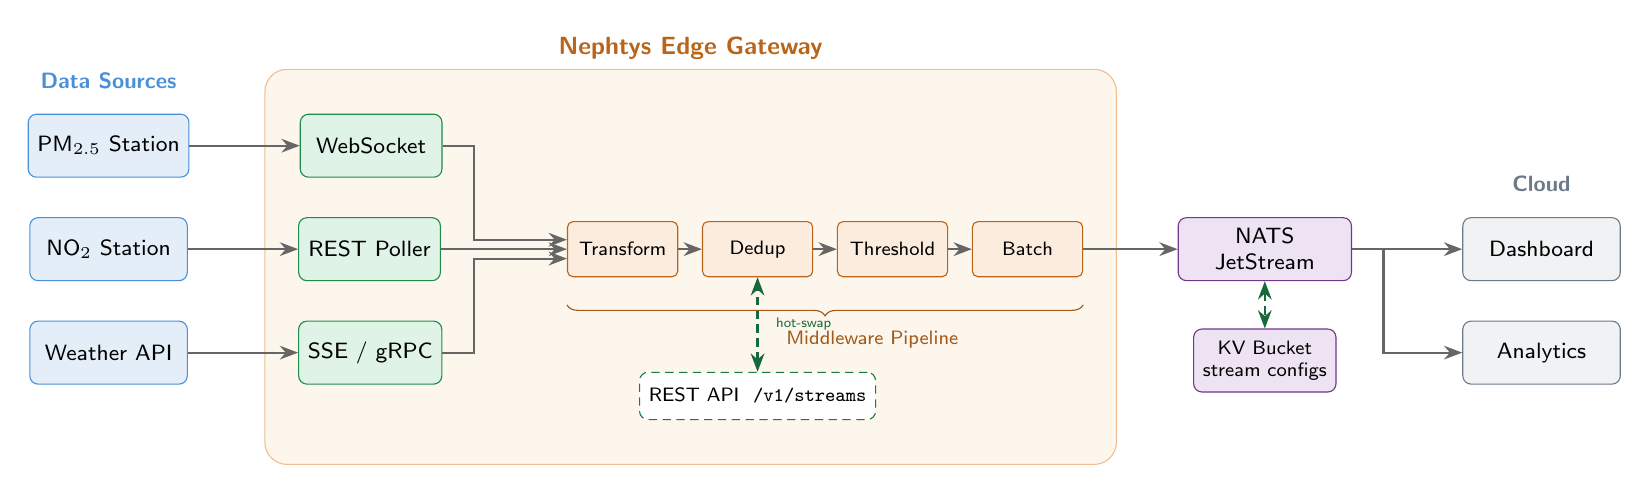
\begin{tikzpicture}[
    >=Stealth,
    every node/.style={font=\sffamily\small},
    sensor/.style={
      rectangle, rounded corners=3pt, draw=sensorblue, fill=sensorblue!15,
      minimum width=2.0cm, minimum height=0.8cm, align=center,
      font=\sffamily\footnotesize
    },
    conn/.style={
      rectangle, rounded corners=3pt, draw=conngreen!80!black, fill=conngreen!15,
      minimum width=1.8cm, minimum height=0.8cm, align=center,
      font=\sffamily\footnotesize
    },
    mw/.style={
      rectangle, rounded corners=2pt, draw=pipeorng!80!black, fill=pipeorng!15,
      minimum width=1.4cm, minimum height=0.7cm, align=center,
      font=\sffamily\scriptsize
    },
    broker/.style={
      rectangle, rounded corners=3pt, draw=natspurp!80!black, fill=natspurp!15,
      minimum width=2.2cm, minimum height=0.8cm, align=center,
      font=\sffamily\footnotesize
    },
    cloud/.style={
      rectangle, rounded corners=3pt, draw=cloudgray, fill=cloudgray!10,
      minimum width=2.0cm, minimum height=0.8cm, align=center,
      font=\sffamily\footnotesize
    },
    api/.style={
      rectangle, rounded corners=3pt, draw=conngreen!70!black,
      fill=white, minimum width=1.8cm, minimum height=0.6cm,
      align=center, font=\sffamily\scriptsize, densely dashed
    },
    arr/.style={->, thick, color=black!60},
    harr/.style={<->, thick, color=conngreen!60!black, densely dashed},
  ]

  \node[sensor]                  (s1) {PM$_{2.5}$ Station};
  \node[sensor, below=0.5cm of s1] (s2) {NO$_2$ Station};
  \node[sensor, below=0.5cm of s2] (s3) {Weather API};
  \node[above=0.2cm of s1, font=\sffamily\footnotesize\bfseries, text=sensorblue]
    {Data Sources};

  \node[conn, right=1.4cm of s1] (c1) {WebSocket};
  \node[conn, right=1.4cm of s2] (c2) {REST Poller};
  \node[conn, right=1.4cm of s3] (c3) {SSE / gRPC};

  \node[mw, right=1.6cm of c2] (m1) {Transform};
  \node[mw, right=0.3cm of m1]  (m2) {Dedup};
  \node[mw, right=0.3cm of m2]  (m3) {Threshold};
  \node[mw, right=0.3cm of m3]  (m4) {Batch};

  \node[api, below=1.2cm of m2] (api) {REST API~~\texttt{/v1/streams}};

  \node[broker, right=1.2cm of m4] (nats) {NATS\\JetStream};
  \node[broker, below=0.6cm of nats, minimum width=1.8cm,
        font=\sffamily\scriptsize] (kv) {KV Bucket\\{\scriptsize stream configs}};

  \node[cloud, right=1.4cm of nats]  (cl1) {Dashboard};
  \node[cloud, below=0.5cm of cl1]   (cl2) {Analytics};
  \node[above=0.2cm of cl1, font=\sffamily\footnotesize\bfseries, text=cloudgray]
    {Cloud};

  \begin{scope}[on background layer]
    \node[draw=pipeorng!50, fill=edgebg, rounded corners=8pt,
          fit=(c1)(c3)(m1)(m4)(api),
          inner xsep=12pt, inner ysep=16pt,
          label={[font=\sffamily\small\bfseries, text=pipeorng!80!black]
                 above:Nephtys Edge Gateway}] (edgebox) {};
  \end{scope}

  \draw[decorate, decoration={brace, amplitude=4pt, mirror}, pipeorng!70!black]
    ($(m1.south west)+(0,-0.35)$) -- ($(m4.south east)+(0,-0.35)$)
    node[midway, below=6pt, xshift=0.6cm, font=\sffamily\scriptsize, text=pipeorng!70!black]
    {Middleware Pipeline};

  \draw[arr] (s1) -- (c1);
  \draw[arr] (s2) -- (c2);
  \draw[arr] (s3) -- (c3);
  \draw[arr] (c2) -- (m1);
  \draw[arr] (c1.east) -- ++(0.4, 0) |- ($(m1.west)+(0, 0.12)$);
  \draw[arr] (c3.east) -- ++(0.4, 0) |- ($(m1.west)+(0,-0.12)$);
  \draw[arr] (m1) -- (m2);
  \draw[arr] (m2) -- (m3);
  \draw[arr] (m3) -- (m4);
  \draw[arr] (m4) -- (nats);
  \draw[harr] (nats) -- (kv);
  \draw[harr] (api.north) -- ($(m2.south)+(0,0)$)
    node[midway, right=3pt, font=\sffamily\tiny, text=conngreen!60!black] {hot-swap};
  \draw[arr] (nats) -- (cl1);
  \draw[arr] (nats.east) -- ++(0.4,0) |- (cl2);

\end{tikzpicture}%
}

  \caption{Nephtys system architecture. Sensor data flows left-to-right through protocol connectors and a composable middleware pipeline before publication to NATS JetStream. The REST API enables runtime hot-swapping of pipeline configurations.}
  \label{fig:arch}
\end{figure*}

\subsection{Fault-Tolerant Ingestion}

Each data source is managed by a \emph{connector} abstraction that encapsulates the protocol-specific logic (WebSocket, REST poller, SSE, webhook, gRPC). In a Smart City deployment~\cite{zanella2014iot}, connectors may simultaneously ingest high-frequency air-quality readings via WebSocket from a local sensor gateway and poll a municipal open-data REST API for meteorological context.

All connectors implement automatic reconnection with \textbf{exponential backoff} (initial delay 1\,s, capped at 30\,s). This prevents accidental denial-of-service flooding when an upstream sensor gateway reboots or loses connectivity, a common occurrence on battery-powered or solar-powered field nodes. On connection loss the connector transitions to a \emph{reconnecting} state and resumes ingestion transparently once the source is available again.

\subsection{Zero-Infrastructure Persistence}

Edge nodes frequently lack the resources to run a relational database or even an embedded key-value store alongside the application. Nephtys addresses this by using \textbf{NATS JetStream}~\cite{nats2024} as both the event transport and the configuration store. Published sensor events are stored in a durable JetStream stream with configurable retention (default: 72 hours), surviving process restarts without data loss. Active stream configurations are serialized in a JetStream Key-Value bucket (\texttt{nephtys\_streams}). On startup, the Stream Manager reads all persisted entries and re-registers the corresponding connectors and pipelines, achieving full state recovery with no external dependencies.

This design means Nephtys and NATS are the \emph{only two processes} required on an edge node, a minimal footprint suitable for single-board computers such as the Raspberry Pi~4. All connectors support TLS-encrypted upstream connections (WSS, HTTPS), and the management REST API is protected by Bearer-token authentication, preventing unauthorized pipeline reconfiguration.

\subsection{Edge Pipeline for Bandwidth Reduction}

The central component is the \textbf{Pipeline Middleware} engine. Before an event reaches the broker, it traverses a chain of composable middleware stages, each independently configurable per stream:

\begin{itemize}
  \item \textbf{Transform}: Extracts only the relevant fields from nested JSON payloads using dot-notation path mapping, reducing per-event payload size.
  \item \textbf{Dedup}: Computes the FNV-64a hash~\cite{fnv2019} of each payload and blocks duplicates within a configurable time-to-live window.
  \item \textbf{Threshold}: Passes an event only if the absolute change in a numerical field exceeds a configurable delta (e.g., $\Delta\mathrm{PM}_{2.5} \geq 1.0\;\mu\mathrm{g/m^3}$), filtering out sensor noise.
  \item \textbf{Batch}: Buffers events and flushes them as a single aggregated message at a configurable interval or batch size, reducing per-message overhead.
  \item \textbf{Filter} and \textbf{Enrich}: Drop events not matching specified types, or inject static metadata tags.
\end{itemize}

The pipeline configuration is a JSON object attached to each stream registration and can be \textbf{hot-swapped at runtime} via a \texttt{PUT /v1/streams/\{id\}/pipeline} REST call. Internally, the active pipeline handler is stored behind a Go \texttt{atomic.Pointer}, so the swap is lock-free and takes effect on the next event with sub-millisecond latency. This allows operators to tighten or relax filtering thresholds in response to air-quality alerts without interrupting data flow.

% ================================================================
\section{Evaluation Scenario}

We evaluate Nephtys in an urban air-quality monitoring scenario representative of a Smart City edge deployment. All source code, the sensor simulator, and an automated benchmark script are publicly available in the companion repository\footnote{Companion material: \url{https://github.com/AndreaBozzo/uic2026-nephtys}; Nephtys source: \url{https://github.com/AndreaBozzo/Nephtys}} to allow full reproducibility of the results presented below.

\subsection{Experimental Setup}

Nephtys runs on a host machine; NATS JetStream, Prometheus, and Grafana are co-deployed via Docker Compose. Two classes of data sources feed the system:

\begin{enumerate}
  \item \textbf{Synthetic sensor streams}: A lightweight WebSocket-based simulator (\texttt{sensor-sim}) generates air-quality readings for 20~virtual stations at 2\,Hz, producing ${\sim}40$~events/s. Each event contains PM$_{2.5}$, PM$_{10}$, NO$_2$, temperature, and humidity values with configurable jitter and a 30\% duplicate ratio, modeling the redundancy typical of low-cost particulate-matter sensors.
  \item \textbf{Real-world open data}: Five REST poller streams ingest live measurements from the Open-Meteo weather and air-quality APIs~\cite{openmeteo2024} for three cities in Calabria (Cosenza, Catanzaro, Reggio Calabria) and from a Sensor.Community~\cite{sensorcommunity2024} citizen PM sensor near Gioia Tauro, polled every 30--60\,seconds.
\end{enumerate}

The full middleware pipeline is configured as: Transform (5 fields extracted), Dedup (TTL\,=\,30\,s, cache\,=\,500), Threshold (path\,=\,\texttt{pm25}, $\delta$\,=\,1.0\,$\mu$g/m$^3$), Batch (size\,=\,50, flush\,=\,5\,s).

\subsection{Results}

Table~\ref{tab:results} reports metrics from two experiments: (a)~a 5-minute synthetic run with 20 virtual stations at 2\,Hz (${\sim}40$ events/s, 30\% duplicate ratio), and (b)~a 30-minute real-data run with five REST poller streams hitting the Open-Meteo~\cite{openmeteo2024} and Sensor.Community~\cite{sensorcommunity2024} APIs.

\begin{table}[t]
  \centering
  \caption{Benchmark results: baseline vs.\ full pipeline on synthetic and real-data streams.}
  \label{tab:results}
  \begin{tabular}{@{}lrrr@{}}
    \toprule
    \textbf{Metric} & \textbf{Baseline} & \textbf{Pipeline} & \textbf{Reduction} \\
    \midrule
    \multicolumn{4}{@{}l}{\emph{Synthetic streams (20 stations, 5\,min)}} \\
    \quad Bytes published     & 2,759,750 & 856,228  & 69.0\% \\
    \quad Messages published  & 12,120    & 149      & 98.8\% \\
    \midrule
    \multicolumn{4}{@{}l}{\emph{Real-data streams (5 APIs, 30\,min)}} \\
    \quad Bytes published     & 146,931 & 23,653  & 83.9\% \\
    \quad Messages published  & 275     & 30      & 89.1\% \\
    \midrule
    RSS memory          & \multicolumn{2}{c}{28.6\,MB} & ---    \\
    \bottomrule
  \end{tabular}
\end{table}

\textbf{Synthetic workload.} The bandwidth reduction is decomposed by middleware stage using the Prometheus counter \texttt{events\_dropped\_by\_pipeline\_total}. Of the 12,120 events ingested, \textbf{Dedup} dropped 3,713 (78.7\% of all drops), i.e.\ redundant identical readings within the 30\,s TTL window. \textbf{Threshold} filtered an additional 1,005 events (21.3\% of drops), corresponding to sub-delta PM$_{2.5}$ fluctuations. The remaining 7,402 events were compacted by \textbf{Batch} into 149~messages (avg.\ 50 events per message), and \textbf{Transform} reduced the per-event payload from 227 to 116~bytes (49\% reduction).

\textbf{Real-data workload.} On the five live API streams polled over 30~minutes, 155 of 275~events were dropped by dedup and 90 by threshold, reducing published messages to 30 (89.1\%). The byte reduction was even higher (83.9\%) because Transform extracts 5--6~fields from the ${\sim}$465-byte Open-Meteo JSON responses. The four Open-Meteo streams each achieved ${>}$99\% bandwidth reduction; the Sensor.Community stream, which reports genuinely new readings every ${\sim}$70\,s, showed a lower but still meaningful 21\% reduction via dedup alone.

\textbf{Resilience.} When the sensor simulator process is killed, the WebSocket connector detects the disconnection and enters exponential backoff (1\,s, 2\,s, 4\,s, \ldots, capped at 30\,s). After the simulator is restarted, Nephtys reconnects automatically within 1--2\,s. No crash or manual intervention is required; ingestion simply pauses and resumes.

\textbf{Hot-reload latency.} Issuing a \texttt{PUT} request to change the threshold delta completes in under 16\,ms (including the full HTTP round-trip). The atomic pointer swap ensures the new pipeline takes effect on the very next event, with no loss or reordering.

Fig.~\ref{fig:dashboard} shows the Grafana dashboard captured during the benchmark, displaying the real-time bandwidth and event reduction ratios.

\begin{figure}[t]
  \centering
  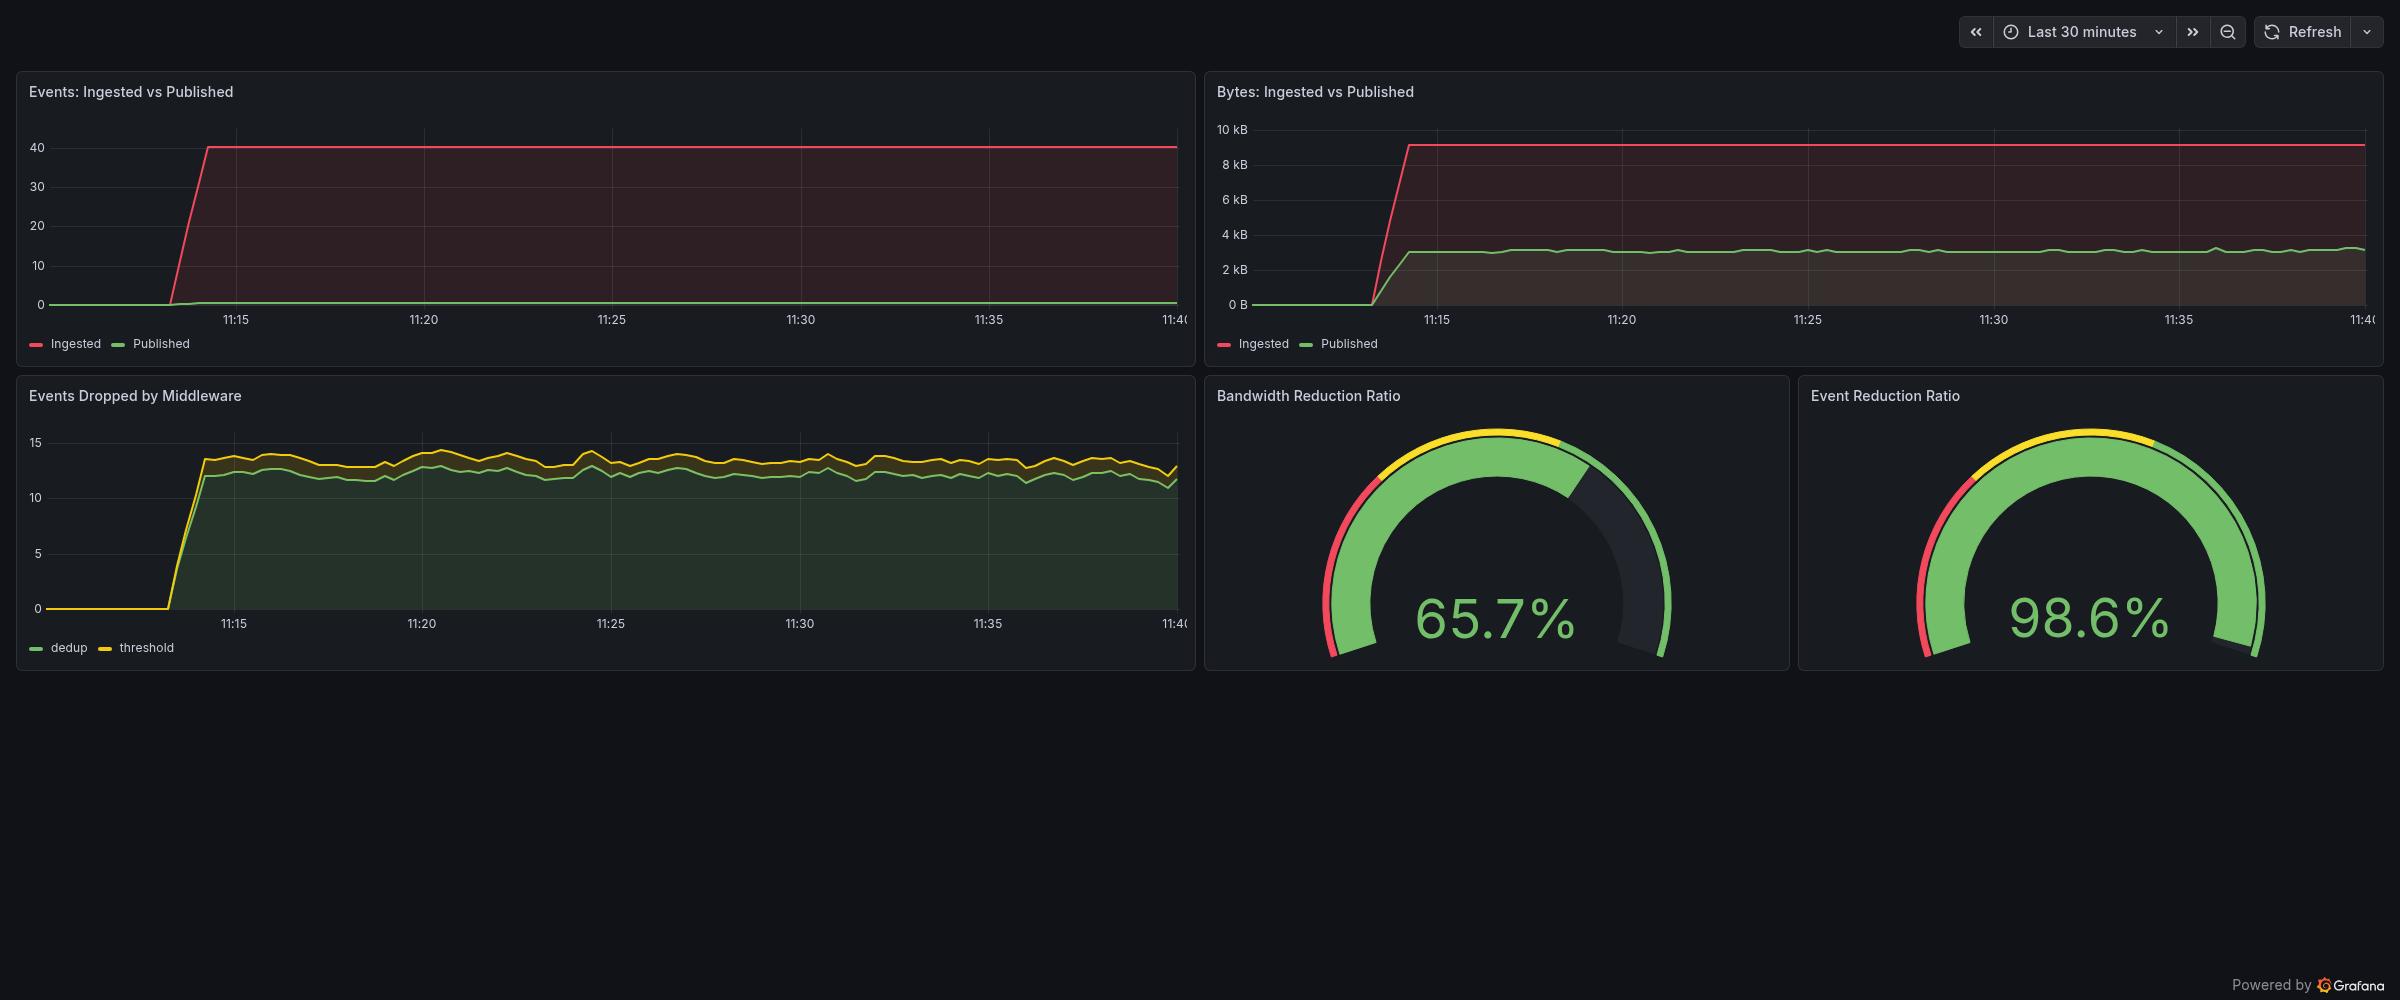
\includegraphics[width=\columnwidth]{fig_grafana_dashboard.png}
  \caption{Grafana dashboard during a mixed workload (synthetic + real-data streams), showing ingested vs.\ published rates, per-middleware drop breakdown, and reduction gauges (65.7\% bandwidth, 98.6\% events).}
  \label{fig:dashboard}
\end{figure}

% ================================================================
\section{Related Work and Conclusions}

\subsection{Related Work}

Several frameworks target data processing at the IoT edge, but each carries trade-offs that Nephtys addresses. \textbf{EdgeX Foundry}~\cite{edgex2024} is a comprehensive, microservice-based edge platform whose multi-container deployment model imposes considerable resource overhead (typically ${>}$\,512\,MB RAM). \textbf{Eclipse Kura}~\cite{kura2024} provides an OSGi-based Java runtime for IoT gateways, but its JVM dependency conflicts with the minimal-footprint goal. \textbf{MQTT bridges}~\cite{mqtt2019} offer lightweight forwarding but no processing capability. \textbf{Node-RED}~\cite{nodered2024} enables visual flow-based programming for IoT, but its Node.js runtime results in higher memory consumption and lower throughput.

Nephtys differentiates itself through the combination of (i)~a compiled, single-binary Go~\cite{go2024} deployment with ${<}$\,30\,MB RSS, (ii)~a per-stream middleware pipeline that is hot-swappable at runtime via REST API, and (iii)~zero-infrastructure persistence using NATS JetStream~\cite{nats2024} as the sole backing store.

\subsection{Conclusions}

This paper presented Nephtys, a lightweight edge connector that demonstrates how compiled languages and lightweight message brokers can enable bandwidth-efficient telemetry ingestion for Smart City sensor networks. By shifting deduplication, transformation, and threshold filtering to the edge through declaratively configurable middleware pipelines~\cite{assuncao2018stream}, the system achieves 69--84\% reduction in upstream bandwidth and up to 98.8\% reduction in message count on both synthetic and real urban air-quality workloads, all within a memory footprint of 28.6\,MB.

The runtime reconfigurability of the pipeline, enabled by atomic pointer swapping, allows operators to adapt filtering behavior to changing conditions (e.g., tightening thresholds during pollution alerts) without interrupting data flow, a capability absent from existing lightweight edge solutions.

Future work includes the addition of an MQTT connector to support legacy sensor deployments, the integration of lightweight ML-based anomaly detection as a pipeline middleware stage, and the federation of multiple Nephtys instances across a city-wide edge mesh for coordinated, distributed intelligence at the urban periphery.

% ================================================================
\bibliographystyle{IEEEtran}
\bibliography{references}

\end{document}
